\subsection{Difficulties with symbolic dynamics}

In the previous section we discretized the continuous time system via a Poincar\'e map, and studied some examples of (quasi)-periodic orbits directly. To study the discrete system further, a typical approach taken is to construct a Markov partition, and to pass to a symbol space with a shift map. Providing a Markov partition in our case proved more complicated than expected. We need a better understanding of the (un)stable manifold of a point $x\in\Sout$. Furthermore, it is not exactly clear how to ``carve'' up $\Sout$ in the first place.

To avoid this, we decided to introduce the Lempel-Ziv complexity as described in \cite{LZ76}. The Lempel-Ziv complexity operates on finite length sequences of symbols by applying a compression algorithm, the complexity of the original sequence is then quantified by the result of the compression. Partitioning $\Sout$ and prescribing an alphabet is still an issue but we first discuss Lempel-Ziv.

\subsection{The Lempel-Ziv compression algorithm}

To explain the algorithm, we use a series of examples, as in the paper \cite{Kaspar1987EasilyCM}. We are not interested in the technicalities of the original paper by Lempel and Ziv, so we only cite results when needed.

Consider a sequence $s=s_1s_2\dots s_n$ of length $n\in\mathbb N$, the algorithm decides what is the smallest number of ``words'' in the sequence necessary for reconstruction. Suppose we have reconstructed $s$ up to the index $k<n$ and the word counter is $c$, that is, we have $s_1\dots s_k$. For the next iteration, the algorithm decides what is the largest $k<\ell\le n$ such that the subsequence $s_{k+1}\dots s_\ell$ appears at some index in $s_1\dots s_{\ell-1}$. Once this $\ell$ is found, the word counter is increased to $c+1$. If $\ell =n$, then the algorithm terminates, otherwise the process is repeated with $s_1\dots s_{\ell+1}$. We provide an example below. The $\cdot$ is used as a delimiter between words, the top line indicates the longest subsequence found at each iteration, and the bottom line shows where they can be found.

\begin{align*}
\overline{0}1011010001101110010
&\xrightarrow{(1)}0\cdot\overline{1}011010001101110010 \\
&\xrightarrow{(2)}\underline{0\cdot1}\cdot\overline{01}1010001101110010 \\
&\xrightarrow{(3)}\underline{0\cdot1\cdot0}11\cdot\overline{010}001101110010 \\
&\xrightarrow{(4)}0\cdot1\cdot\underline{011\cdot01}00\cdot\overline{01101}110010 \\
&\xrightarrow{(5)}0\cdot1\cdot011\cdot0\underline{100}\cdot011011\cdot\overline{100}10 \\
&\xrightarrow{(6)}\underline{0}\cdot1\cdot011\cdot0100\cdot011011\cdot1001\cdot\overline{0} \\
&\xrightarrow{(7)}0\cdot1\cdot011\cdot0100\cdot011011\cdot1001\cdot0 \\
\end{align*}
At the start, we scan from the left, and notice we have never encountered a $0$, so for step (1) we add $0$ on its own. Next, we encounter $1$ for the first time, and add it in step (2). Next, we see that we have encountered $01$, so we add $011$. Notice, how we ignore the delimiter between words. We indicate the rest of the steps without commentary. Once the algorithm terminates, we see that the number of words is 7, so the complexity of this sequence is $7$.

The complexity is not normalized to $[0,1]$, this is not needed since we only ever consider finite length sequences and those clearly have bounded LZ complexity. Comparing two sequences of varying length, the sequences can have the same complexity, though it is expected that the longer sequence will have a higher complexity. Now, that we have an idea how the Lempel-Ziv (LZ) complexity is computed, we can discuss how LZ captures the regularity (or lack of it) in symbolic dynamics.

Suppose for now, we have a map taking orbits of a system to elements of a symbol space, then we can distinguish three levels for LZ complexity: high, low, and intermediate. Since LZ is not normalized, and varies depending on the length of the sequences we consider, it is best to work with sequences of the same length. Furthermore, provided we fix the length, the boundary between cases is not well defined. A rule of thumb is to judge the level by comparison, for each system there will be an average complexity for a sampling of orbits, so low complexity will be well below the average and high will be well above. The average can be skewed depending on the sampling but this should be discussed on a case by case basis.

We can characterize the orbits by their complexity as follows:

\begin{itemize}
\item If a sequence has high complexity that means we cannot reconstruct the sequence from a small number of words. A word corresponds to some substructure in the orbit, and if there are many unique substructures, we should expect the orbit to be disorganised or chaotic.
\item If the complexity is low, meaning very few words are required to reconstruct the sequence, then the corresponding orbit should be regular and repetitive. So, we would expect a (quasi)-periodic orbit to have a low complexity.
\item For intermediate complexity the scenario can be mixed. The orbit can appear mostly random with intermitent sections of structure. The orbit can also be (quasi)-periodic but with a significantly longer period for recurrence than an orbit with low complexity.
\end{itemize}
Of course, this in not formal reasoning and just an intuitive approach. An example where our reasoning breaks down is if a periodic orbit requires $n$ symbols to describe one period and we only sampled $n$ symbols. In this case the complexity can look high, instead of low as one would expect from a periodic orbit. In practice, we find it easy to work around these limitations as will be shown in the next section.

\subsection{Partitioning the Poincar\'e section and compression}

Now, to utilize LZ we need a map from orbits to symbol sequences. We have many options here from the partitioning of the Poincar\'e section to the size of the alphabet, and we do not necessarily need to use a Markov partition for LZ to give us good results. We decided to use a relaxed approach.

Consider the system in the plane, now via the pullback from the torus, $\Sout$ becomes the outward-pointing boundary of circles centered at lattice points. We know by \cref{lem:SoutToSin} that a point $x\in\Sout$ is mapped to another point on $\partial S$. We disregard the exact point and velocity of $P_\text{oi}(x)$ and only record the relative position of the new circle we intersected. For example, if we have initially $x,v = (1/2,5/6,0,1)$, so we are on the circle centered at $(1/2,1/2)$, then $P_\text{oi}(x,v)=(1/2,7/6,0,1)$ which is on the circle centered at $(1/2,3/2)$, the symbol we record here is $(1/2,3/2)-(1/2,1/2)=(0,1)$. We see immediately there are infinitely many such pairs $(n,m)\in\mathbb Z^2$ that we can attain. We argue that this is not a problem for computing LZ, since there can only be finitely many of these pairs in a finite sequence anyway, i.e, the complexity of a sequence is capped by its length. Another way to look at it: the pairs $(n,m)\in\mathbb Z^2$ are words constructed using a finite alphabet $i\in\mathbb Z$ with $|i|\le 9$, so we can unpair the coordinates and work with a stream of integers.

An example to get the idea. Consider the orbit in \cref{subfig:periodicorbit1}, the orbit goes down, left, up, right, and repeats, so in symbols that is
\begin{align*}
((0,-1),(-1,0),(0,1),(1,0),\dots),
\end{align*}
and this pattern repeats indefinitely. To compute LZ, we take a finite slice, for example the first 20 symbols. If computed correctly, LZ should be 5, we record the first 4 symbols as words, and the 5th word is the rest of the 16 symbols, since they just repeat the first 4. The complexity in \cref{subfig:periodicorbit2} is also $5$, though in \cref{subfig:periodicorbit3} and \cref{subfig:periodicorbit4} the complexity is 9. We notice also that if we took the first 100 symbols of these orbits, the complexity would still be 5 and 9, respectively, provided they are stable (quasi)-periodic orbits.

\subsection{Examples and thoughts}

We now look at some examples. We find LZ performs well when we compute it for a range of initial conditions and parameters.

Consider again the examples from \cref{subfig:periodicorbit1} and \cref{subfig:periodicorbit2}, the second one was obtained by slightly perturbing the initial position and this hints that the periodic trajectory is stable. We ask now how much can we perturb the initial conditions before we leave the region of stability for this periodic orbit. We take $R=1/3, b=3$ and compute LZ for the family of intial conditions:
\begin{align*}
x= \left(\frac{1}{2}+\sqrt{R^2-y^2},\delta\right),\quad v = \left(1,0\right),\qquad \text{for } y\in [-0.32,0.32]+\frac{1}{2},
\end{align*} 
that is, we keep the velocity the same, and we sweep the right half-circle centered at $(1/2, 1/2)$. We report the results in \cref{subfig:LZsweepY}. We see that the region spans values of $y$ roughly in $[0.346, 0.653]$. We also notice there are some dips outside the region of stability. Out of curiosity we plot the orbit of the far left dip in \cref{fig:sensitive_trajectory}, interestingly, the orbit at first is scattered and then gets trapped between four bumps. Later, we computed more iterations of the orbit and noticed it eventually leaves the four bumps, so it seems the orbit came close to the stable region but did not enter it.

In \cref{subfig:LZsweepb} we instead fix the initial conditions $x,v=(5/6,1/2,1,0)$ and vary $b\in(0.001,10)$. We see that near $b=4$, LZ is consistently high, while for $b<4$ there are some dips: the dips that contain $b=3$ and $b=3(\sqrt2-1)\approx1.25$ should correspond to the regions of stability for the orbit in \cref{subfig:periodicorbit1}, and \cref{subfig:periodicorbit3}, respectively. There are other dips in the plot, however we ignore them, they could either be comparatively small stable regions or one of the few ``false positives'' that we discussed before.

\begin{figure}[!th]
\centering
\begin{subfigure}[t]{0.49\textwidth}
\centering
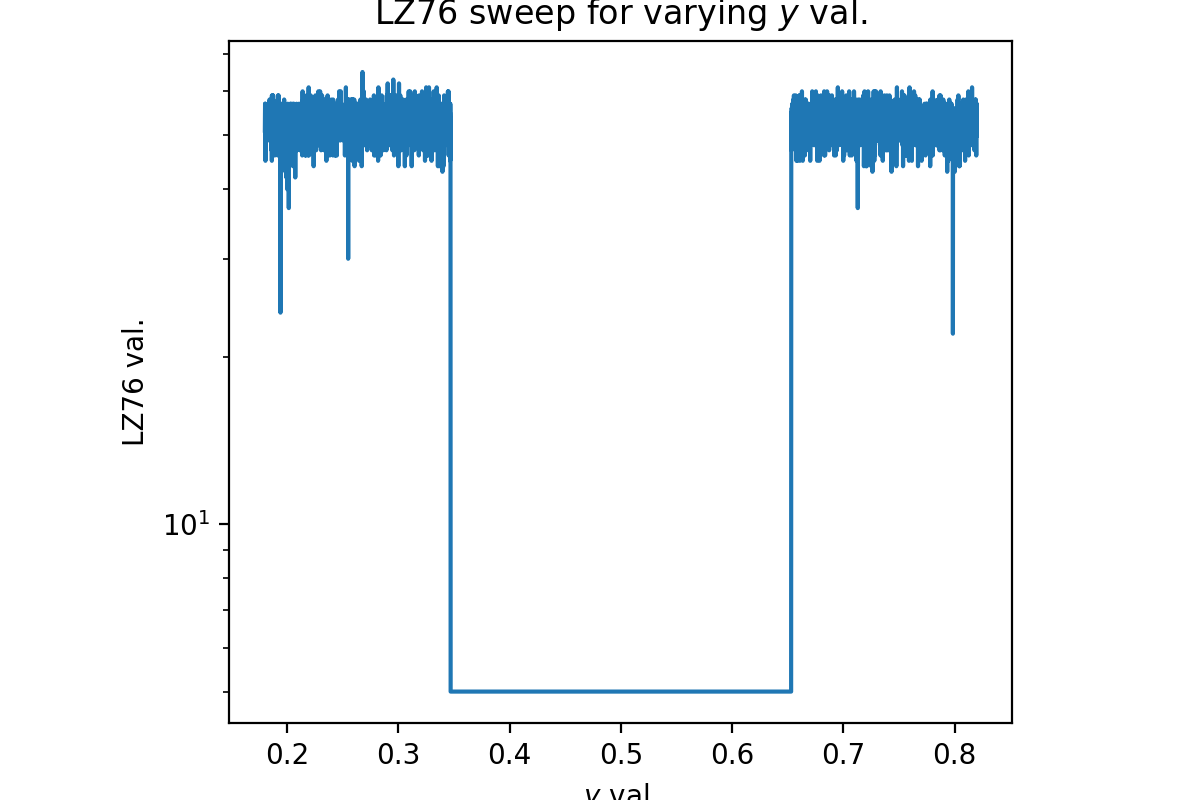
\includegraphics[width=\textwidth, trim={0cm 0 0cm 0}, clip]{LZ_y_sweep.png}
\caption{}
\label{subfig:LZsweepY}
\end{subfigure}
%
\begin{subfigure}[t]{0.49\textwidth}
\centering
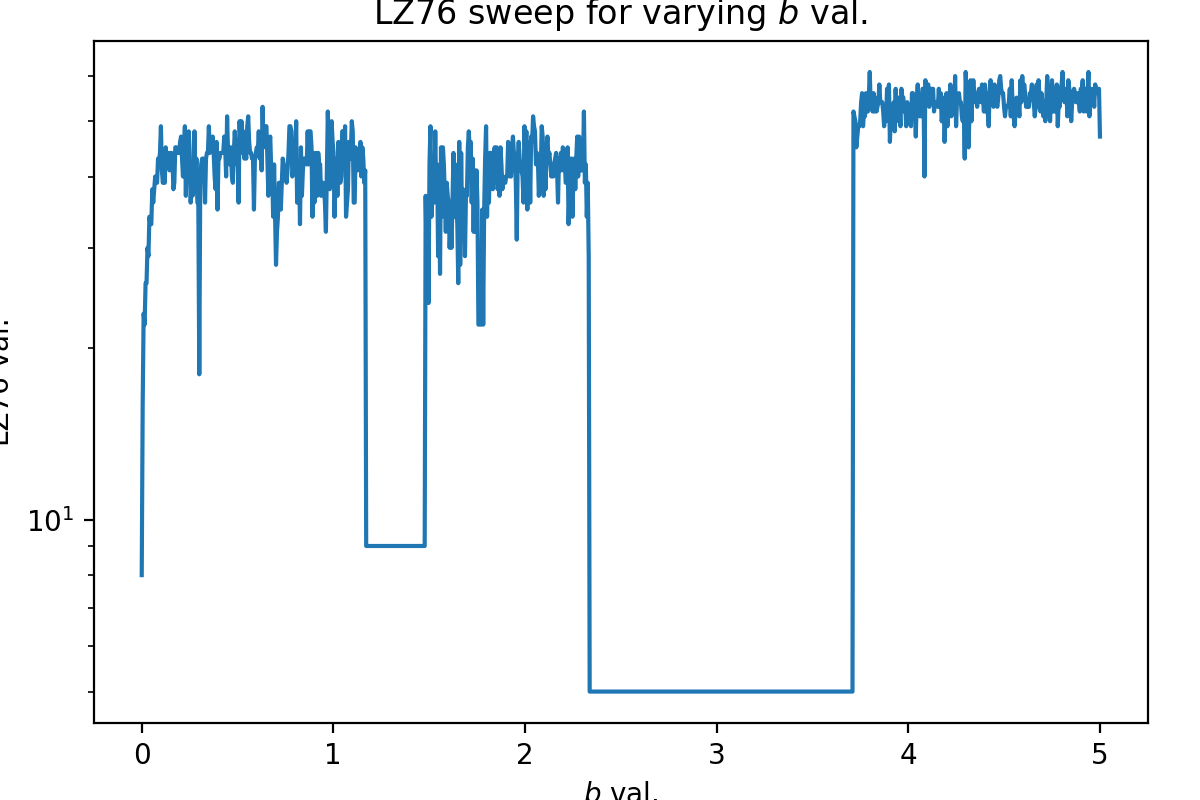
\includegraphics[width=\textwidth, trim={0cm 0cm 0cm 0cm}, clip]{LZ_b_sweep.png}
\caption{}
\label{subfig:LZsweepb}
\end{subfigure}
\caption{}
\label{fig:LZsweep1d}
\end{figure}


If instead we sample a grid of points on the Poincar\'e section $\Sout$, we can compute LZ as in \cref{subfig:LZpoincaresectionb3}. We only compute LZ for a strip of the Poincar\'e section, specifically, for $\theta\in[-\pi/4,\pi/4]$, since the rest of the picture can be reconstructed via translation. This corresponds to the 4-fold rotational symmetry of a square lattice, that is, if we rotate $\mathbb R^2$ at the origin by an angle of $n*\pi/2$ for $n=0,\dots, 3$, the lattice of circles stays the same, and the resulting dynamics are the same as well.

In \cref{subfig:LZpoincaresectionb3} we compute LZ for $R=1/3$ and $b=3$. We see a large stable ``eye'' at $(\theta, \varphi)=(0,0)$. This is not unexpected, since we've seen evidence for a large stable region in \cref{subfig:LZsweepY}. Besides the eye, we see some lines that have intermediate complexity, and on those either lie unstable periodic orbits or special occurances like \cref{fig:sensitive_trajectory}. We include some close ups of the eye: the top left corner of the eye where we notice some obvious fractal behavior, and another spot along the boundary of the eye. We must note again that the emerging features in the images are sensitive to varying the depth of simulation. When attempting to plot the close ups, for example, the second one, we noticed that more yellow strips would appear and their width would increase the longer we simulated. The deeper we simulate, the more the boundary moves, which is not unreasonable since we capture more information.

\begin{figure}[!th]
\centering
\hfill
\begin{subfigure}[h]{0.49\textwidth}
\centering
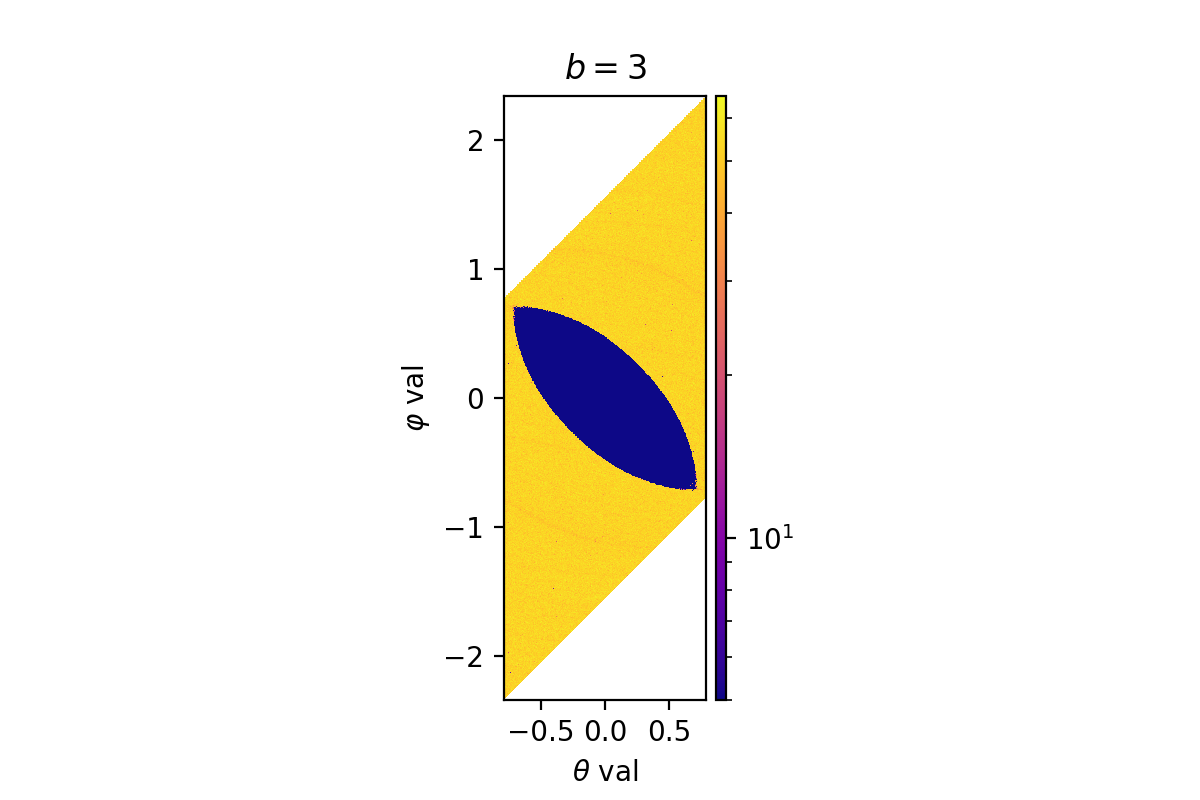
\includegraphics[width=\textwidth, trim={5cm 0cm 4cm 0cm}, clip]{LZ_th_ph_b_3_sweep.png}
\caption{}
\label{subfig:LZpoincaresectionb3}
\end{subfigure}
%
\begin{subfigure}[h]{0.49\textwidth}
\centering
%\includegraphics[width=\textwidth, trim={0cm 0 0cm 0}, clip]{fig18.png}
%
%\includegraphics[width=\textwidth, trim={0cm 0 0cm 0}, clip]{fig16.png}
%
%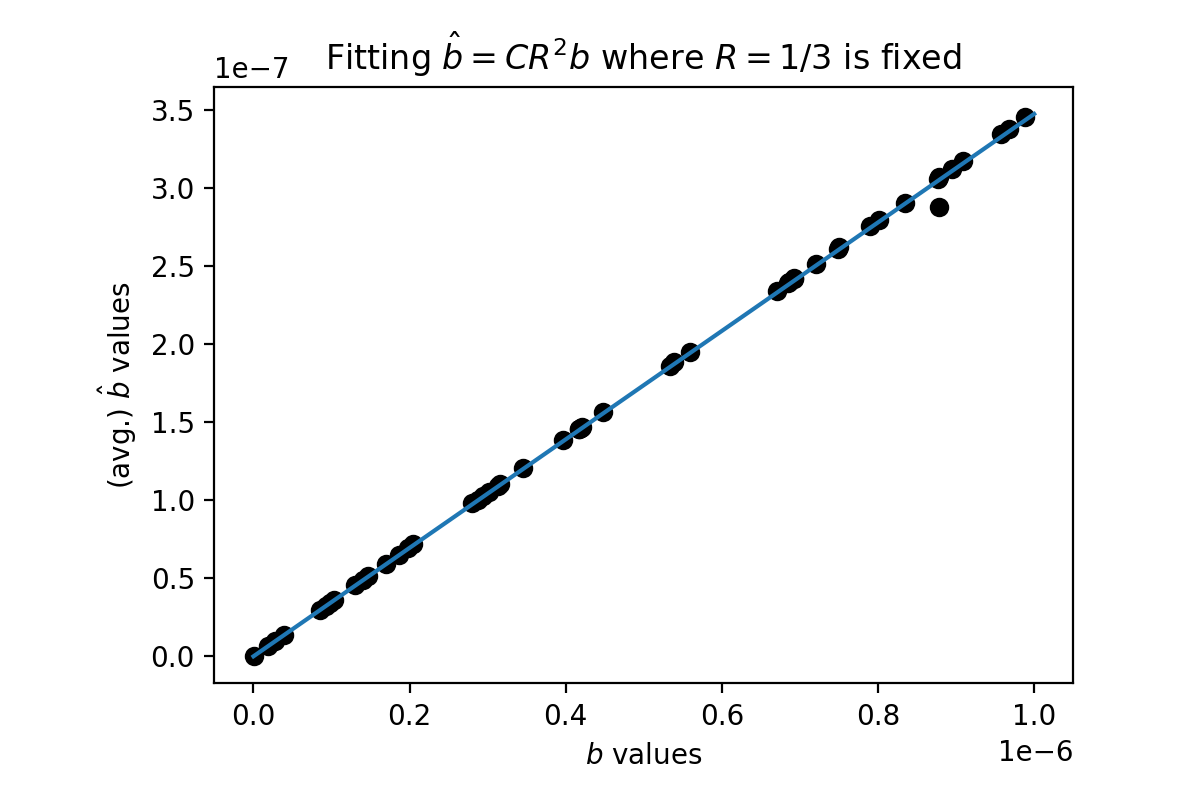
\includegraphics[width=\textwidth, trim={0cm 0 0cm 0}, clip]{kam_approx_line.png}
\caption{placeholder}
\end{subfigure}
\caption{}
\end{figure}


In \cref{subfig:LZpoincaresectionb1242} we plot the same data except $b\approx3(\sqrt2-1)$, so we plot the Poincar\'e section corresponding to \cref{subfig:periodicorbit3}. We notice there are several very stable regions, however by comparing with \cref{subfig:periodicorbit3} they should correspond to the same family of (quasi)-periodic orbits. The shape of the very stable regions is quite different, they are twisted with fractal ``digits''. Besides the large regions there are intermediate complexity regions scattered about, due to their globular shapes we suspect they are also relatively stable.

\begin{figure}[!th]
\centering
\hfill
\begin{subfigure}[h]{0.49\textwidth}
\centering
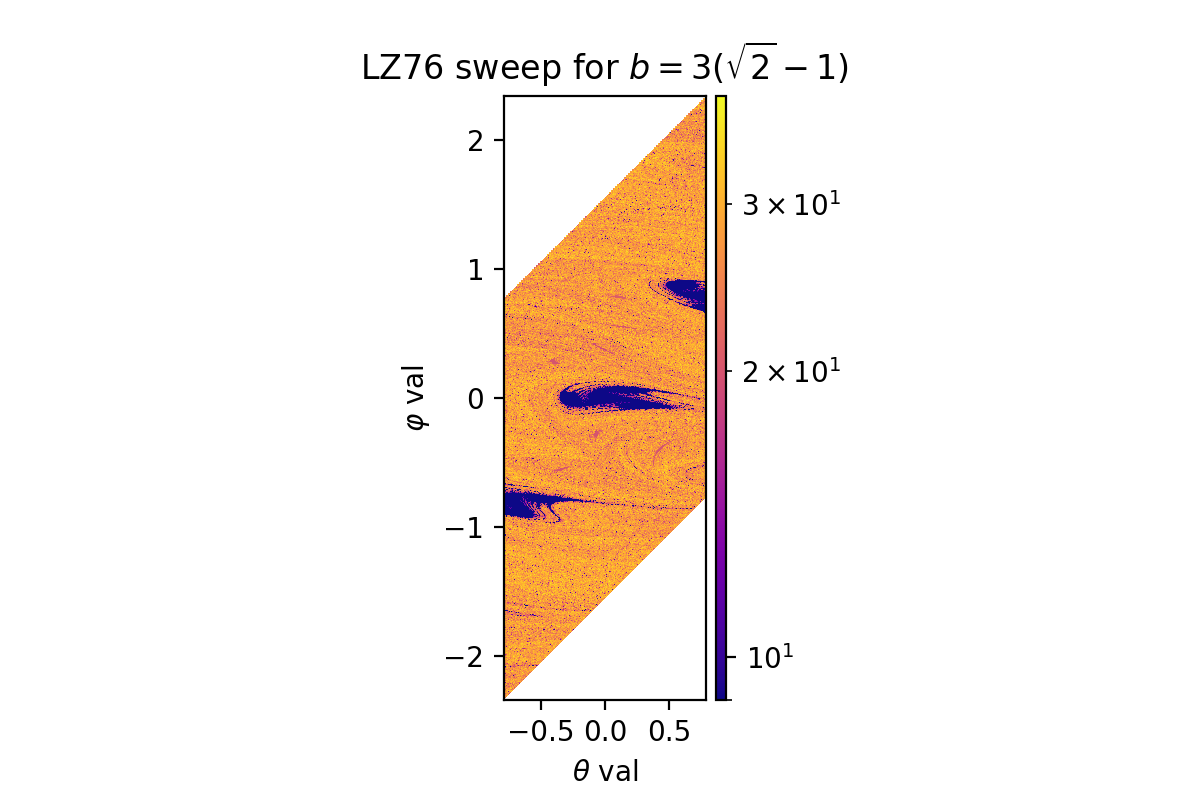
\includegraphics[width=\textwidth, trim={4cm 0cm 4cm 0cm}, clip]{LZ_th_ph_b_3sqrt2-1_sweep.png}
\caption{}
\label{subfig:LZpoincaresectionb1242}
\end{subfigure}
%
\hfill
\begin{subfigure}[h]{0.49\textwidth}
\centering
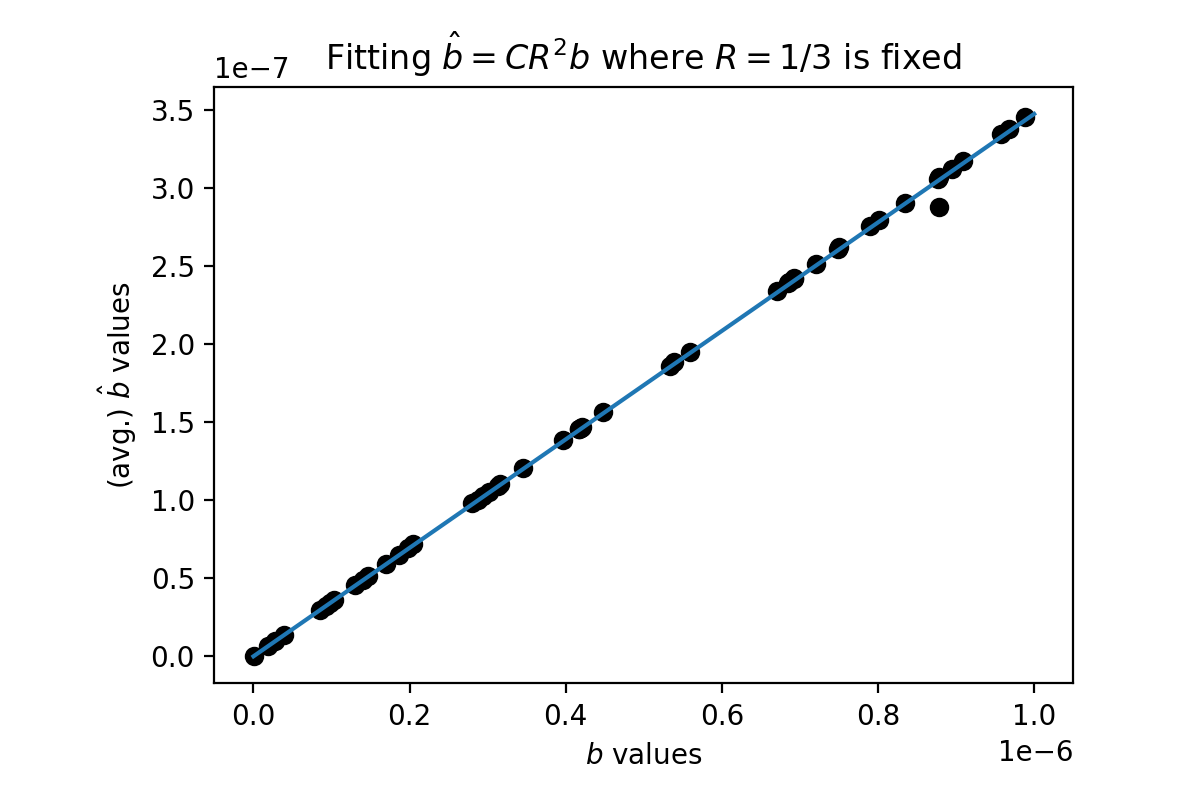
\includegraphics[width=\textwidth, trim={0cm 0 0cm 0}, clip]{kam_approx_line.png}
%
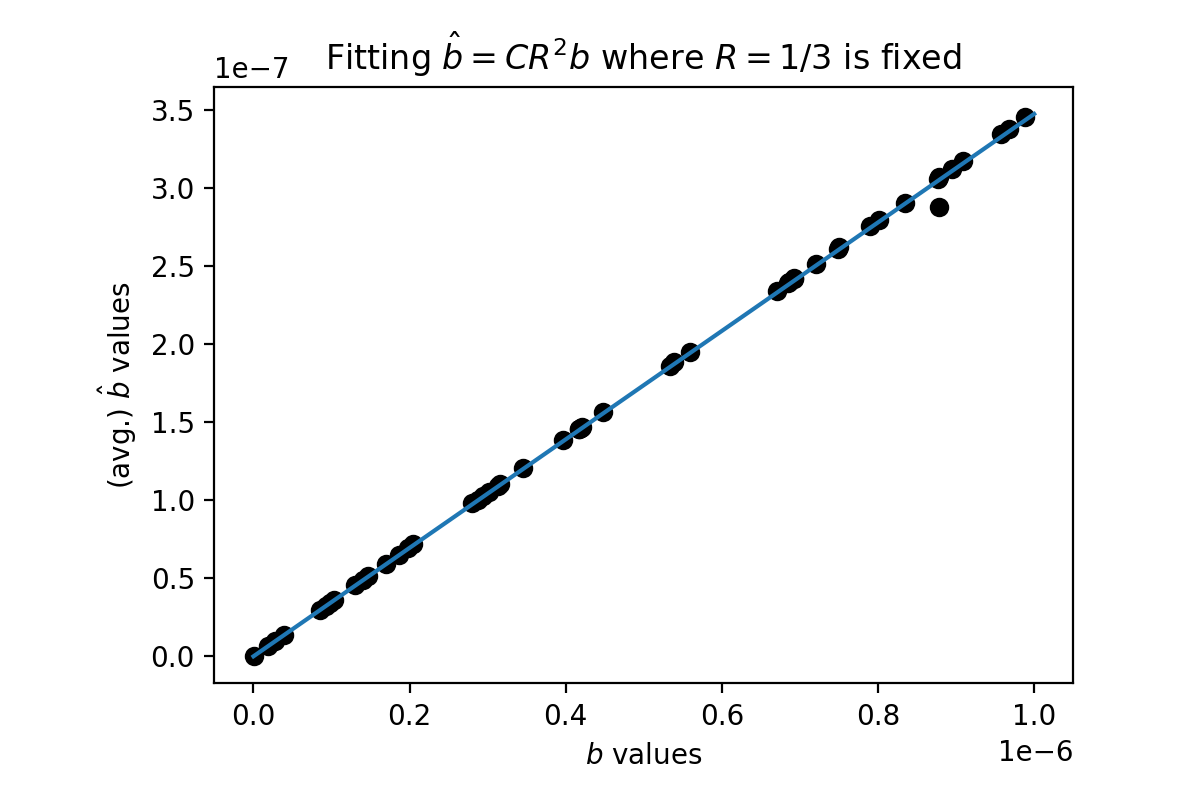
\includegraphics[width=\textwidth, trim={0cm 0 0cm 0}, clip]{kam_approx_line.png}
%
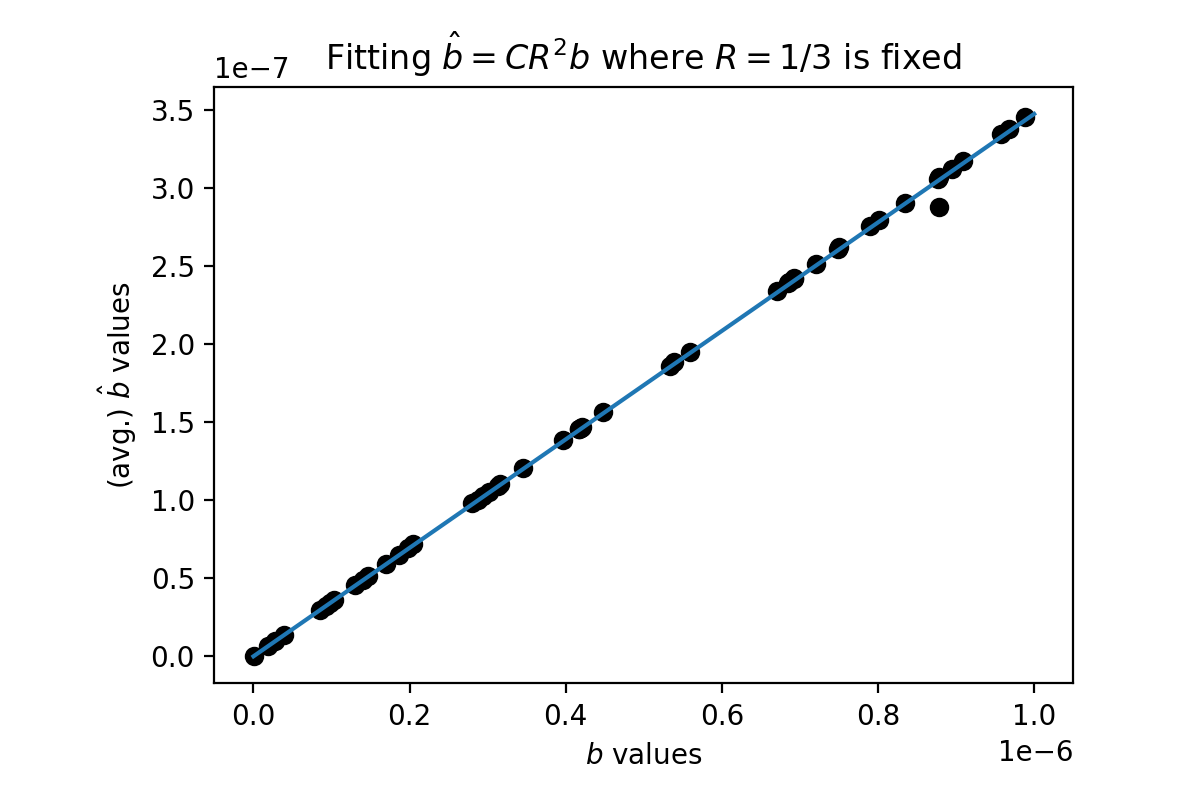
\includegraphics[width=\textwidth, trim={0cm 0 0cm 0}, clip]{kam_approx_line.png}
\caption{placeholder}
\end{subfigure}
\hfill
\caption{}
\end{figure}

In \cref{subfig:LZpoincaresectionb232}, we pick a value of $b=2.32$ and find a range of stable regions. Generally, the shapes are elongated, exaggerated compared to the other figures and it is not clear why this is the case. It can be noticed that there are 3 different colors for the stable regions, indicating there could be 3 different stable orbits here.

\begin{figure}[!th]
\centering
\hfill
\begin{subfigure}[h]{0.49\textwidth}
\centering
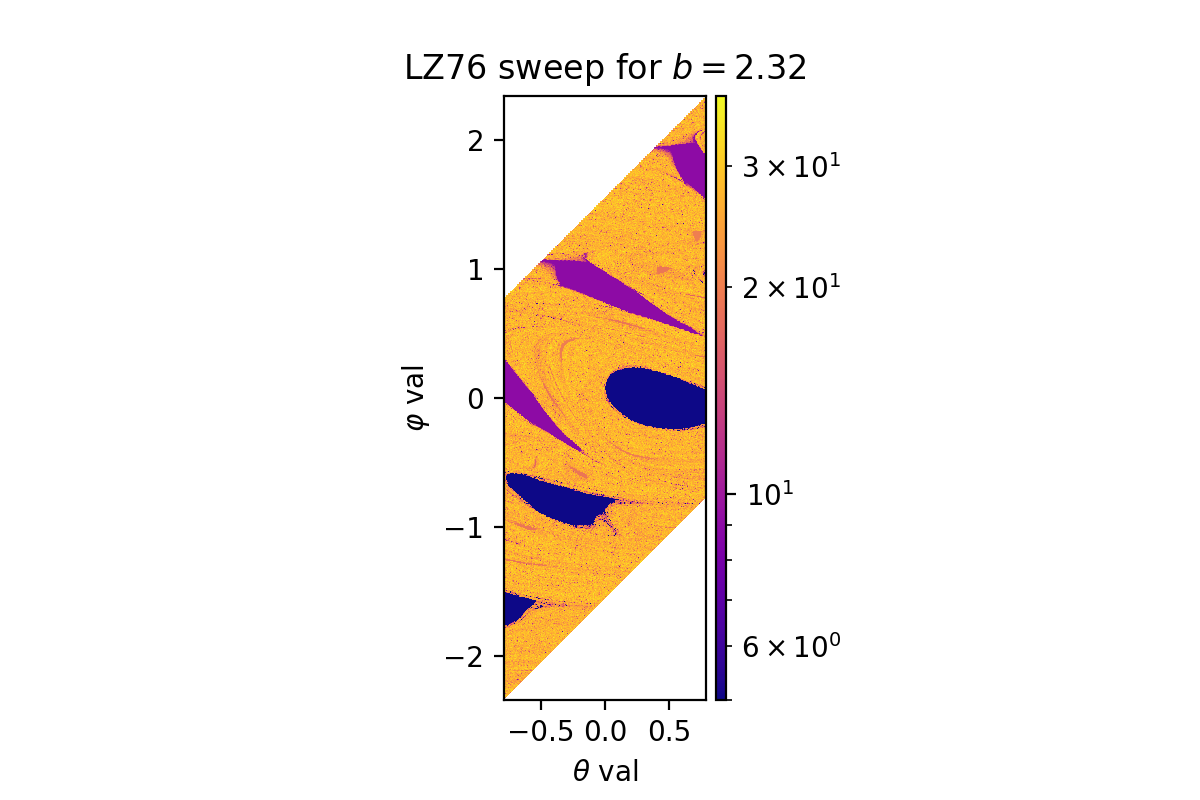
\includegraphics[width=\textwidth, trim={5cm 0cm 4cm 0cm}, clip]{LZ_th_ph_b_2_32_sweep.png}
\caption{}
\label{subfig:LZpoincaresectionb232}
\end{subfigure}
%
\hfill
\begin{subfigure}[h]{0.49\textwidth}
\centering
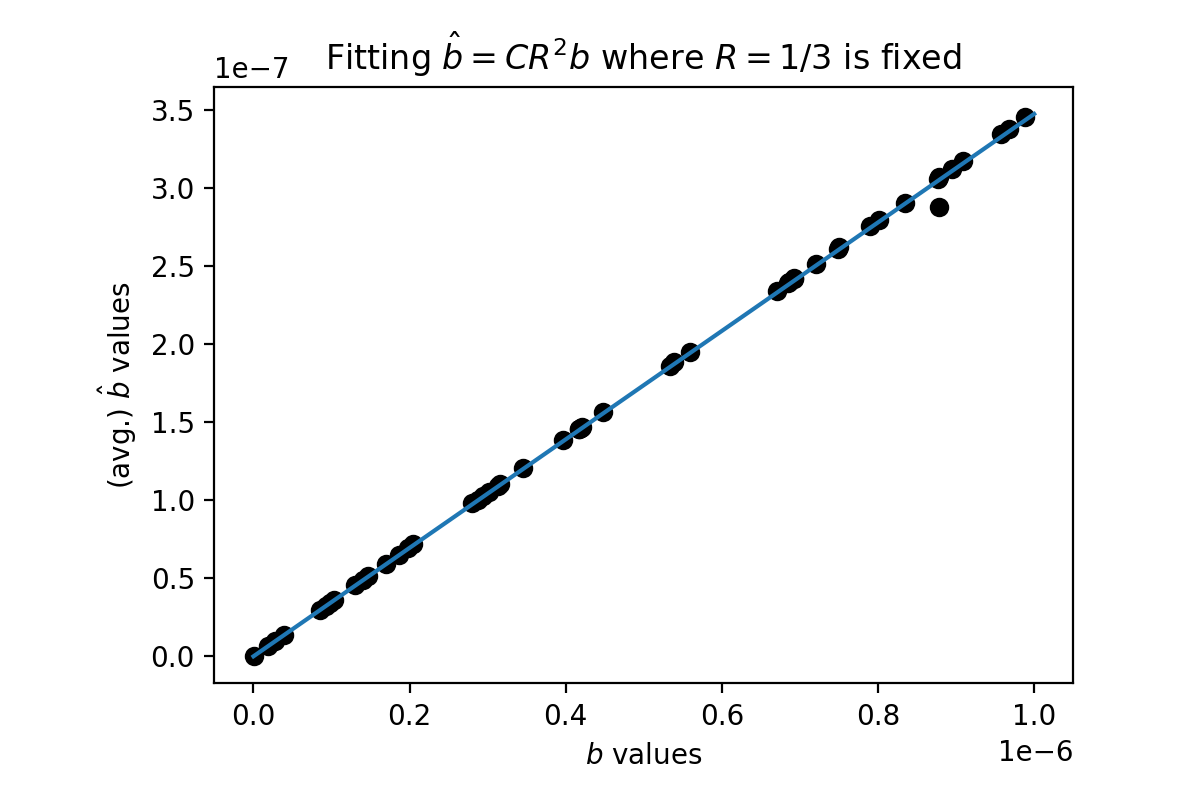
\includegraphics[width=\textwidth, trim={0cm 0 0cm 0}, clip]{kam_approx_line.png}
%
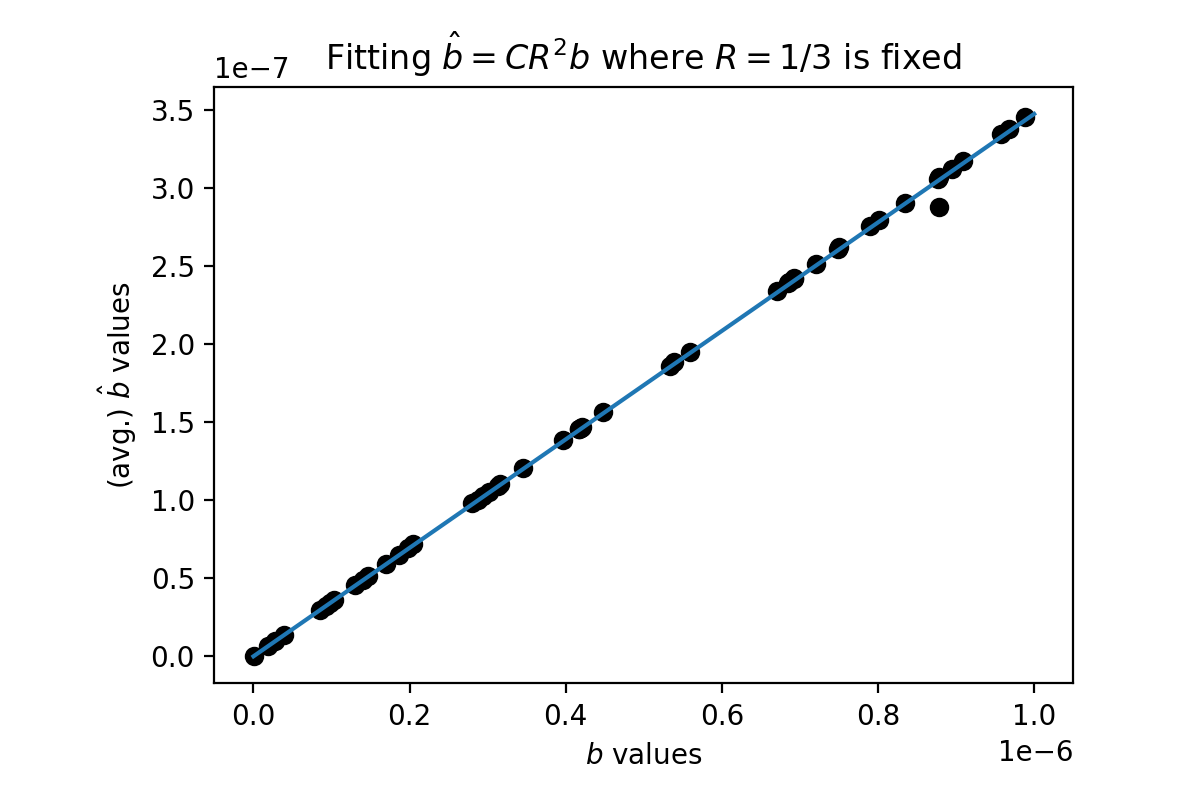
\includegraphics[width=\textwidth, trim={0cm 0 0cm 0}, clip]{kam_approx_line.png}
%
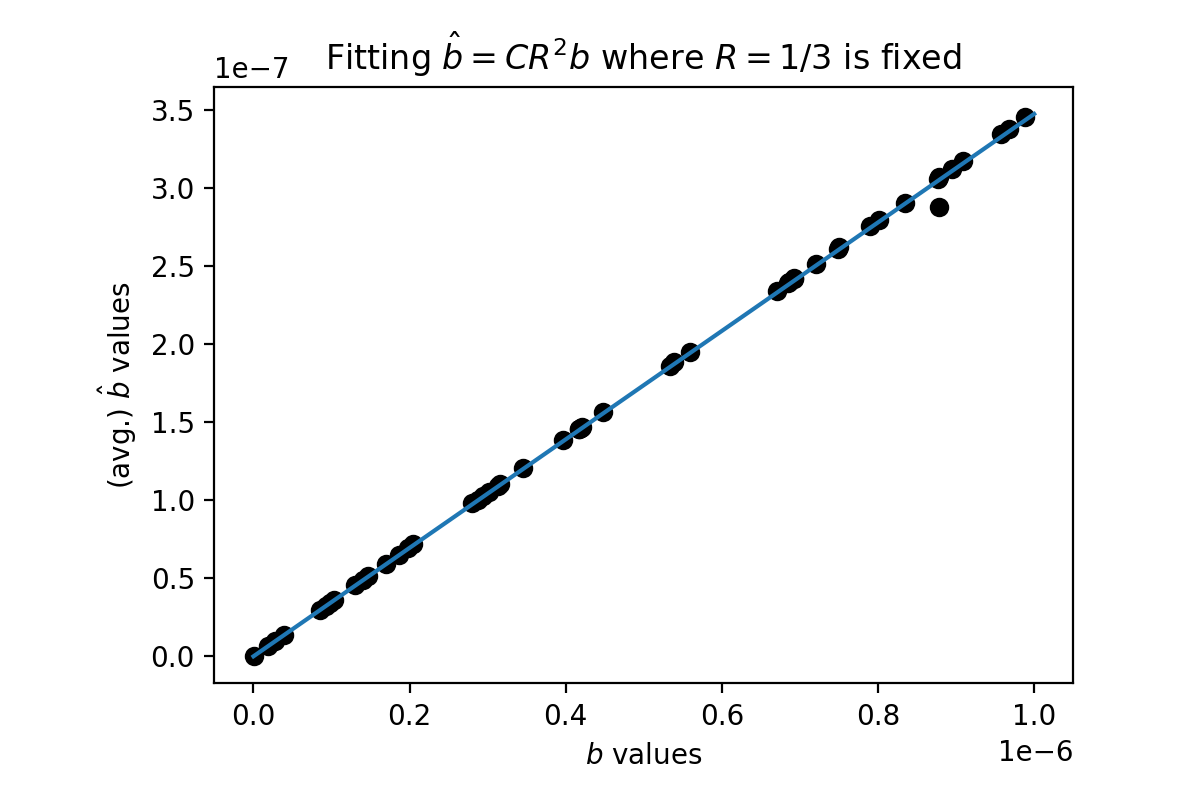
\includegraphics[width=\textwidth, trim={0cm 0 0cm 0}, clip]{kam_approx_line.png}
\caption{placeholder}
\end{subfigure}
\hfill
\caption{}
\end{figure}


\begin{figure}[!th]
\centering
\begin{subfigure}[h]{\textwidth}
\centering
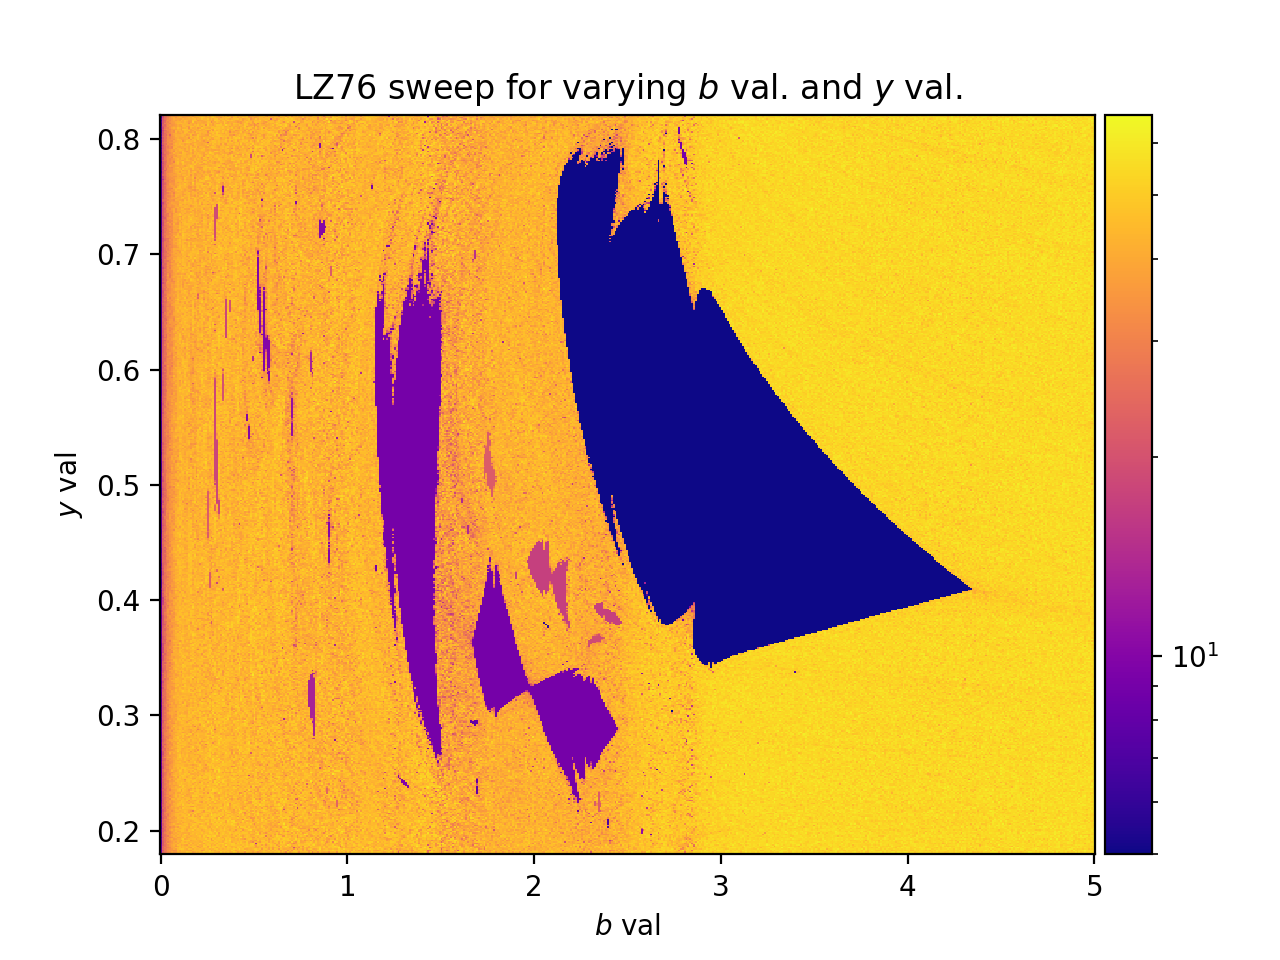
\includegraphics[width=\textwidth, trim={0cm 0cm 0cm 0cm}, clip]{LZ_b_Y_sweep.png}
\caption{}
\label{subfig:LZsweepYandb}
\end{subfigure}
%
\begin{subfigure}[h]{\textwidth}
\centering
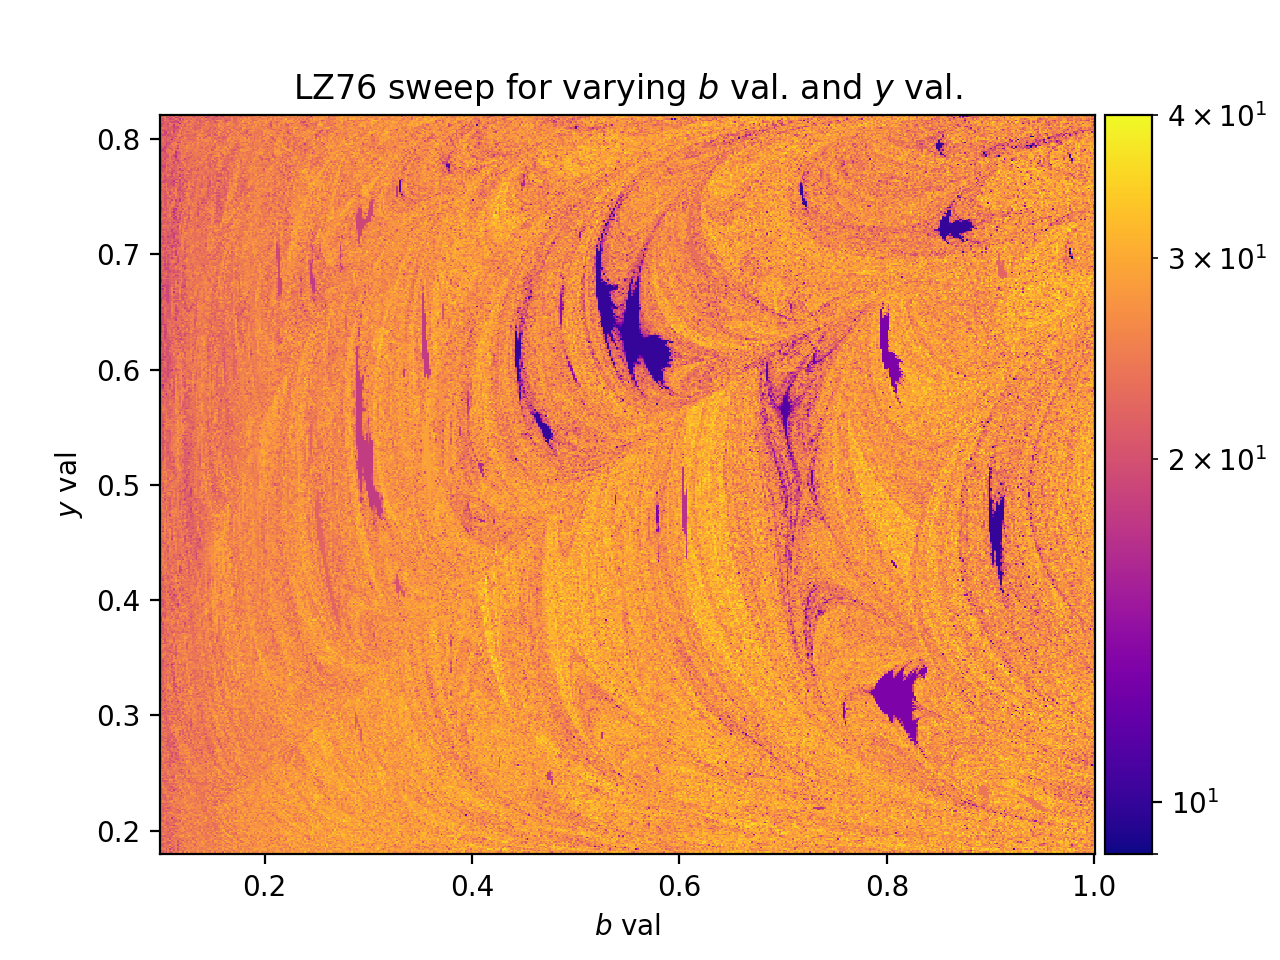
\includegraphics[width=\textwidth, trim={0cm 0cm 0cm 0cm}, clip]{LZ_b_(01_1)_Y_sweep.png}
\caption{placeholder}
\end{subfigure}
\caption{}
\end{figure}